\section{Evaluation}
\label{sec:eval}
In this section, we introduce the dataset, 
baseline and experiment results.


\subsection{Datasets}
%\subsection{Cause-Effects Pairs Corpus}
%%\subsubsection{Cause-Effect Pairs from Novel Corpus}
%To study the causal sentence generation task, we build a new dataset of cause-effect sentence pairs from novels by extracting main and subordinate clauses connected by  causal conjunctions (i.e., ``because'' and ``so''). We first crawl raw novel corpus from Library Genesis\footnote{\url{libgen.is}}, a search engine for articles and books which allows free access. \SN{This website seems have repeated got into copyright disputes, need check if it's good to mention it here.} To maintain the quality of our corpus, we collect a group of prize-winning lists and top-x lists for novels, for example Nobel Prize in Literature and Time Magazine All Time 100 Novels, and limit our crawler to them. The resulting \SN{19000} novels are splitted into around 100 million sentences, which served as our data source after filtering and text cleaning. 
%
%For causal pair extraction, we first collect sentences containing ``because'' or ``so'' by regular expression matching. Those sentences are fed into Stanford CoreNLP~\cite{stanfordcorenlp} tools for tokenization, POS tagging, constituent parsing, dependency parsing and coreference annotation. Following steps are taken to filter out syntactically unwanted or semantically non-causal pairs and to locate the right span of target content:
%\begin{figure}[t!]
%	\centering
%	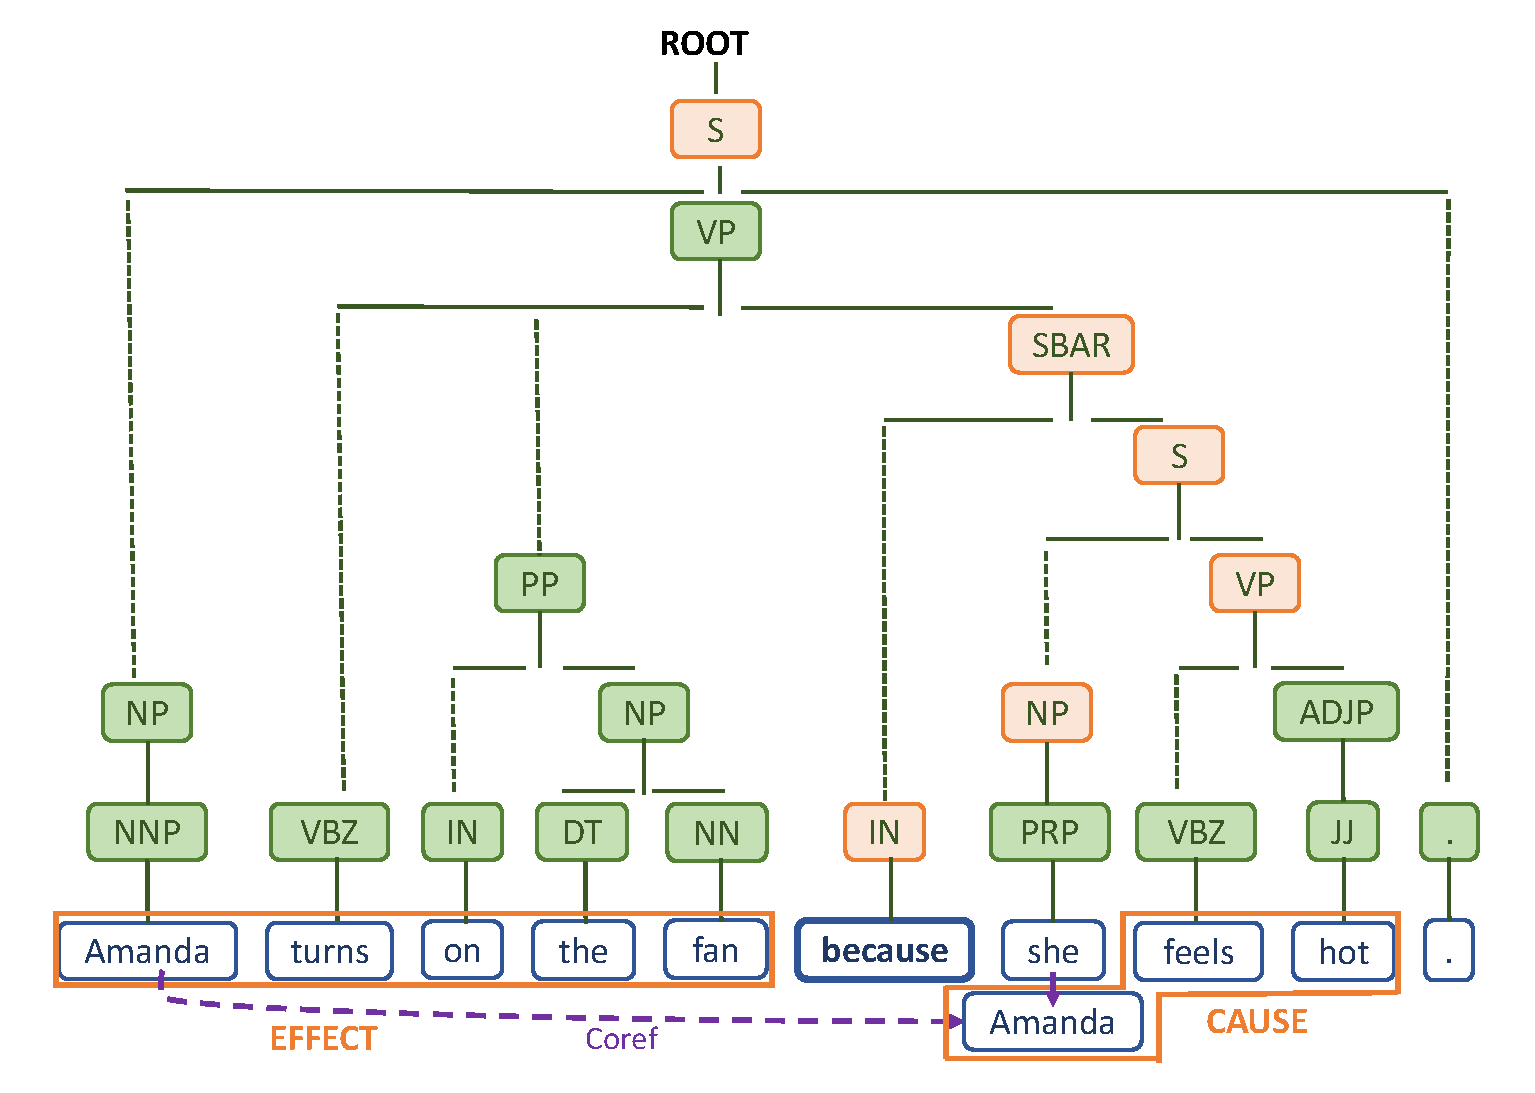
\includegraphics[width=\columnwidth]{parse.pdf}
%	\caption{Cause and effect sentence extracted from a sample sentence along with its constituent parse tree. Nodes coloured in light orange are those critical for syntactical checking in our extraction process.}
%	\label{fig:parse}
%\end{figure}
%\begin{itemize}
%	\item Negation Detection. If the causal conjunction node in dependency tree
%	 has a negation word sibling such as ``not'' and ``n't'', causal relationship 
%	 doesn't exist in this sentence.
%	\item Clause Detection. Since the input and target of our task are both sentences, 
%	cause or effect represented by noun phrases are unwanted. For example, "This is 
%	because of you" has noun as both cause and effect, thus doesn't satisfy our 
%	requirement. We design complicated pattern matching rules on dependency parse 
%	tree and constituent parse trees for this syntactic checking. A simple sample 
%	sentence with its constituent parse tree is shown in \ref{fig:parse}. Basically 
%	we make sure the "because" in the sentence is a subordinate conjunction word 
%	leading a subordinate clause(tagged as `SBAR'), which contains a declarative 
%	sentence(`S') with subject(`NP') and predicate(`VP'). \SN{not complete here. 
%		Jessie may want to say may about this.}
%	\item Span Selection. Sentences passing the previous steps must already have 
%	main clause root node and subordinate clause root node identified in constituent 
%	parse tree. In this step we confirm the spans of cause/effect sentence based on 
%	the root nodes' spans to remove punctuations and unwanted  sentence constituents.
%	\item (Partial) Coreference Resolution. The order of cause/effect span is determined by the 
%	causal conjunction. Take ``because'' as an example, the order is always ``EFFECT 
%	because CAUSE'', resulting in representative mention in effect sentence but 
%	pronouns in cause. Therefore, we substitute pronouns in subordinate clause with 
%	the representative mention in main clause for each causal pair to enable bidirectional 
%	inference. We don't do coreference resolution on the whole sentence to avoid unnecessary repetition. 
%\end{itemize}
%After performing those steps to all sentences in novel corpus, we get \SN{477644} unique 
%cause-effect pairs. \SN{maybe more statisticas here?}

\subsubsection{Test Dataset: COPA}
To better understand the performance of our model against related research, we also use 
the Choice of Plausible Alternatives (COPA) 
as test dataset, which is a widely-attempted causal reasoning benchmark. It consists
of one thousand multiple-choice questions.
Each question is composed of a premise and two alternatives,
where the task is to select the more plausible alternative as a
cause (or effect) of the premise. \SN{how we used it in this paper.}

\subsection{Baselines}
There are four baselines in our experiments.
One is to select causes (or effects) based on premise 
from Cause-Effects Pairs Corpus. 
In details, given a premise and its attribute (cause or effect), 
we rank premises with the same attribute as given premise
in Cause-Effects Pairs Corpus by cosine similarity 
and select top $10$. We can get corresponding causes (or effects)
of these $10$ premises. We rank these causes (or effects) by
causality strength between them and premises, and select cause (or effect)
with best causality strength score.
Others are introduced in \secref{sec:approach}:
CNN seq2seq model, global causal attention and
causal easy attention fusion. 



\subsection{Evaluation Metrics}
In this section, we introduce the evaluation metrics used in 
our experiments.

\textbf{BLEU} scores~\cite{PapineniRWZ02}, includes BLEU-1 and BLEU-2,
which combines modified n-gram precisions and sentence brevity penalty:

\begin{equation}
\small BLEU = \min(1,\exp(1-\frac{r}{c})) \cdot \sum_{n=1}^{N}(w_{n}p_{n})
\end{equation}

where $r$ is the sum of the best match lengths 
for each generated and corresponding reference text in the corpus.
and $c$ is the total length of the predicted corpus. 
$w_n=\frac{1}{N}$ is uniform weights. $N$ is based on the type of BLEU, 
for example, $N$ is $2$ for BLEU-2
$p_n$ is modified n-gram precision. To compute this, 
one first counts the maximum number of times a word occurs reference text. 
Next, one clips the total count of each predicted word by its maximum
reference count, adds these clipped counts up, and
divides by the total number of predicted words. 

\textbf{Causality Score for Text} (CST) from predicted text $T_1$
and premise text $T_2$ is computed as \cite{LuoSZHW16}:

\begin{equation}
\small cst(T_{1},T_{2}) = -\log(\frac{\sum_{i \in T_{1}}\sum_{j \in T_{2}}cs(i,j)}{\left| T_{1} \right| + \left| T_{2} \right|})
\end{equation}
\begin{equation}
\small CST(T_{1},T_{2}) = \frac{1}{cst{T_1,T_2}}
\end{equation}
where $cs(i,j)$ is causality strength 
between $i$-th token in $T_1$ and $j$-th token in $T_2$. 
The higher the score, the stronger the causality.

\textbf{Accuracy} (Acc) is evaluation metric for COPA.
We generate cause (or effect) according to the premise in COPA
and select the more ``similar'' alternative based on the similarity
score. We use \textbf{BLEU} as similarity evaluation methods.

\begin{equation}
Acc = \frac{n_{ct}}{N_{all}}
\end{equation}
where $n_{ct}$ and $N_{all}$ denotes
the number of the questions with correct selection
and all questions in COPA respectively.

We use BLEU-1 since it is suitable for generation
of short sequence. It denotes the degree of matching 
predicted texts and premise texts. 
%As relation between cause and effect is many-to-many, 
%we use CS score, which denotes the causality, to supplement
%BLEU-1 score. The reason for using BLEU and CS as similarity
%score is that they respectively indicate the consistency and causality 
%between two text.

\textbf{Human Evaluation} (Human) is used to supplement
BLEU-1 score, as relation between cause and effect is many-to-many.
We randomly sample 300 premises from COPA and 
corresponding causes (or effects) generated
by each model, and manually inspect their causality strength.
Then, we calculate the percentage of the number of each model ranked 
first in causality strength. This estimate the 
ability of models to generate correct causes (or effects) based on permise .

\subsection{Experiments}
\label{sec:exp}

\begin{table}[th]
	\centering
    \small
	\begin{tabular}{|l|c|c|c|c|}
		\hline
		Model &   BLEU-1  & BLEU-2 & CST & Human \\
		\hline
		CNN & 20.84 & 4.06 & 1.87 & \\
		CS  & & & & \\
		ATT+CS & & & & \\
		\hline
		Ours & & & & \\
		\hline
	\end{tabular}
	\caption{BLEU score and Causility strength score on Cause-Effect Pairs Corpus}
	\label{tab:novel}
\end{table}

\begin{table}[th]
	\centering
    \small
	\begin{tabular}{|l|c|c|c|c|c|}
		\hline
		Model &   BLEU-1 & BLEU-2 & CST & Acc & Human\\
		\hline
        unigram-1 & 11.15 & 0.14 & 2.42 & 0.9 & \\
        unigram-2 & 12.35 & -  & 2.80 & 0.80 & \\
        bigram & 13.42 & 0.41 & 2.50 & 0.82 & \\
		\hline
		CNN & & & & & \\
		CS & & & & & \\
		ATT+CS & & & & & \\
		\hline
		Ours & & & & & \\
		\hline
	\end{tabular}
	\caption{BLEU score, Causility strength score and Accuracy on COPA}
	\label{tab:copa}
\end{table}

\begin{table*}[th]
    \centering
    \small
    \begin{tabular}{r|l}%{|p{7cm}|rl|}
    \hline
    \multicolumn{2}{c}{Cause}\\ 
    \hline
    \multicolumn{2}{c}{}\\ 
    \hline
    \multicolumn{2}{c}{Effect} \\
    \hline
    CNN & \\
    \hline
    CS & \\
    \hline
    ATT+CS & \\
    \hline
    Ours & \\
    \hline
    \end{tabular}
    \caption{Given cause to generate effect.}
    \label{tab:cause_exp}
\end{table*}

\begin{table*}[th]
    \centering
    \small
    \begin{tabular}{r|l}%{|p{7cm}|rl|}
    \hline
    \multicolumn{2}{c}{Effect}\\ 
    \hline
    \multicolumn{2}{c}{}\\ 
    \hline
    \multicolumn{2}{c}{Cause} \\
    \hline
    CNN &  \\
    \hline
    CS &  \\
    \hline
    ATT+CS &  \\
    \hline
    Ours &  \\
    \hline
    \end{tabular}
    \caption{Given effect to generate cause.}
    \label{tab:effect_exp}
\end{table*}

